\documentclass[aspectratio=169,xcolor=dvipsnames, t]{beamer}
\usepackage{fontspec} % Allows using custom font. MUST be before loading the theme!
\usetheme{SimplePlusAIC}
\usepackage{hyperref}
\usepackage{graphicx} % Allows including images
\usepackage{booktabs} % Allows the use of \toprule, \midrule and  \bottomrule in tables
\usepackage{svg} %allows using svg figures
\usepackage{tikz}
\usepackage{makecell}
\usepackage{wrapfig}
\usepackage[czech]{babel}
\usepackage{tabularx}
\newcommand{\R}{\mathbb{R}}
\newcommand{\N}{\mathbb{N}}


\title[]{Internet} % The short title appears at the bottom of every slide, the full title is only on the title page
\subtitle{}

\author[Dusart]{Eric Dusart}
\institute[GEVO]{Gymnázium Evolution Jižní Město}
\date{\today}


\begin{document}

\maketitlepage
{
\setbeamertemplate{background}
{
    
\includegraphics[width=\paperwidth,height=\paperheight]{AICStyleData/logos/mene_polygonu_bg.png}
}
\begin{frame}[t]{Obsah}
    \tableofcontents
\end{frame}
}


\section{Historie}
\setbeamertemplate{background}
{
    
\includegraphics[width=\paperwidth,height=\paperheight]{AICStyleData/logos/mene_polygonu_bg.png}
}
\begin{frame}{Historie}
    \vspace{-0.5cm}
    \begin{columns}
    \begin{column}{0.45\textwidth}
    \begin{itemize}
        \item Internet je propojení počítačů celým světem pomocí počítačových sítí. 
        \item Komunikují mezi sebou pomocí rodiny protokolů TCP/IP.
        \item Služby fungující pomocí internetu $\rightarrow$ webové stránky, sociální sítě, chaty, videohovory, e-mail, \ldots
        \item Roku 1969 byla zprovozněna jedna z prvních sítí ARPANET se čtyřmi uzly (USA).
    \end{itemize}
\end{column}
\begin{column}{0.45\textwidth}
    \begin{figure}
        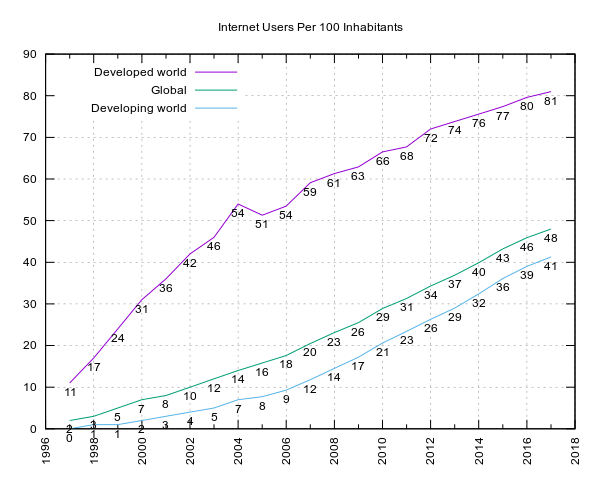
\includegraphics[width=\textwidth]{Internet_users_per_100_inhabitants_ITU}
        \caption{Počet internetových uživatelů na 100 obyvatel.}
    \end{figure}
\end{column}
\end{columns}
\end{frame}

\section{Protokoly}
\subsection{Základní informace}
\setbeamertemplate{background}
{
    
\includegraphics[width=\paperwidth,height=\paperheight]{AICStyleData/logos/mene_polygonu_bg.png}
}
\begin{frame}{Protokoly}
    \vspace{-0.5cm}
    \textbf{\large Základní informace}

    \begin{itemize}
        \item Konvence / standard podle kterého probíhá přenos dat mezi počítači.
        \item Definují formátování, systém, syntax, atd\ldots
        \item Otevřený přístup k protokolům umožňuje rychlejší inovace a rozšiřování informatiky.
        \item Referenční model ISO/OSI nebo skupina protokolů TCP/IP.
    \end{itemize}
\end{frame}

\subsection{HTTP, HTTPS}
\begin{frame}{HTTP, HTTPS}
    \vspace{-0.5cm}
    \textbf{\large Hypertext Transfer Protocol}
    \begin{itemize}
        \item Hypertextové dokumenty obsahují odkazy (omg \href{https://www.youtube.com/watch?v=ZbWIs6z3Thw}{link})
    \end{itemize}
\end{frame}


\section{Internetové služby}
\subsection{Světová široká pavučina}
\setbeamertemplate{background}
{
    
\includegraphics[width=\paperwidth,height=\paperheight]{AICStyleData/logos/mene_polygonu_bg.png}
}
\begin{frame}{Internetové služby: World wide web}
    \vspace{-0.5cm}
    \begin{columns}
    \begin{column}{0.45\textwidth}
        \begin{itemize}
            \item Systém webových stránek zobrazovaných pomocí webového prohlížeče
            \item Používají protokoly HTTP, nebo HTTPS.
            \item Koncem roku 1990 Tim Berners-Lee, zakladatel WWW, spustil první webový server na světě: \href{https://info.cern.ch/}{info.cern.ch}
        \end{itemize}
\end{column}
\begin{column}{0.45\textwidth}
    \begin{figure}
        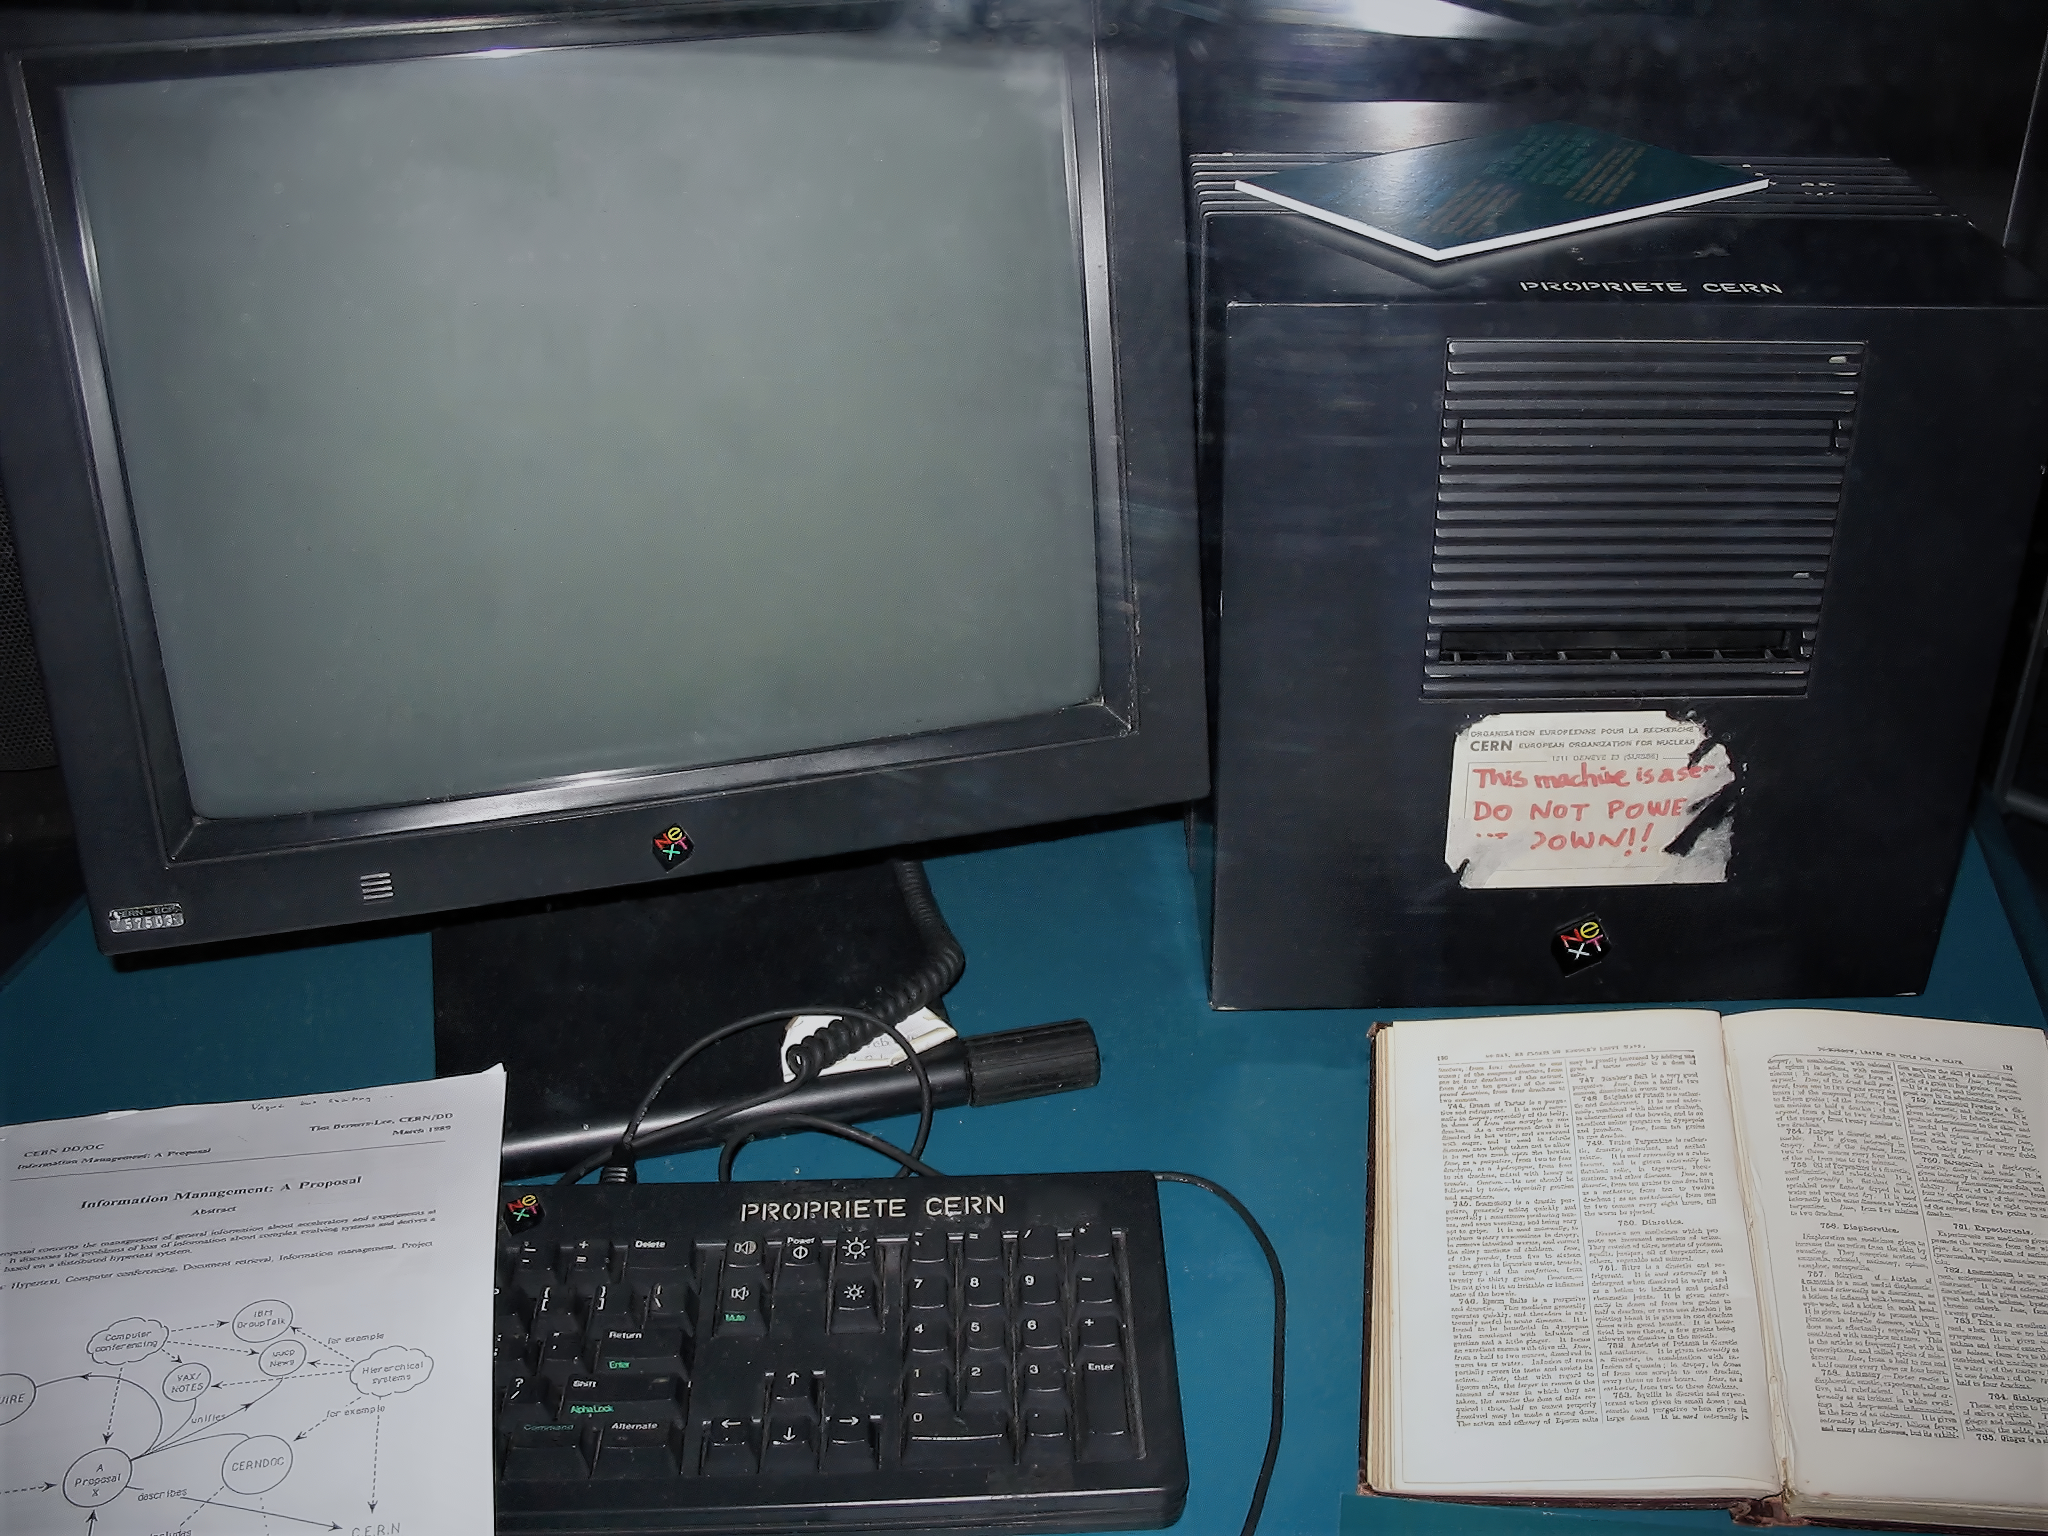
\includegraphics[width=\textwidth]{fw}
        \caption{Setup na kterém běžela první webová stránka.}
    \end{figure}
\end{column}
\end{columns}
\end{frame}

\subsection{e-mail}
\setbeamertemplate{background}
{
    
\includegraphics[width=\paperwidth,height=\paperheight]{AICStyleData/logos/mene_polygonu_bg.png}
}
\begin{frame}{Internetové služby: e-mail}
\vspace{-0.75cm}
\begin{itemize}
    \item Používá protokol SMTP (simple mail transfer protocol), který byl založen roku 1982.
    \item E-mailový klient je program, který posílá e-maily. Ty stahuje z poštovního serveru pomocí protokolů POP nebo IMAC (Ve větších společnostech se někdy používají komerční protokoly, jako například Microsoft Exchange Server.).
\end{itemize}
\textbf{\large{Jak funguje poslání e-mailu?}}
\begin{enumerate}
    \item Odesílatel napíše e-mail. 
    \item Klient pomocí protokolu SMTP pošle zprávu softwaru MTA (mail transfer agend) (může běžet na nějakém serveru nebo přímo na počítači odesílatele).
    \item Program MTA zjistí jméno domény (část e-mailové adresy za @) v DNS (domain name system), aby zjistil mail exchange server.
    \item MTA pošle zprávu mail exchange serveru pomocí protokolu SMPT. Domény mají i záložní mail exchange servery.
    \item Mail exchange server zprávu doručí do schránky adresáta.
    \item Ze schránky adresáta poštovní klient stáhne zprávu pomocí protokolu POP nebo IMAP. 
\end{enumerate}

\end{frame}

\subsection{Volání přes internet}
\setbeamertemplate{background}
{
    
\includegraphics[width=\paperwidth,height=\paperheight]{AICStyleData/logos/mene_polygonu_bg.png}
}
\begin{frame}{Volání pomocí internetu (VoIP)}
    \begin{itemize}
        \item Voice over Internet Protocol.
        \item Pro srozumitelné a spolehlivé volání je nutností zajištění kvality služby $\rightarrow$ Qos (quality of service).
        \begin{itemize}
            \item Rezervace a řízení toků v  telekomunikačních a počítačových sítích, které používají přepojování paketů.
            \item Prioritizace procesů.
        \end{itemize}
        \item Používají se kodeky k úspoře přenosu objemu dat.
        \item Například Skype - ma vlastní closed protokol.
        \item Většinou používají IP protokoly.
    \end{itemize}

\end{frame}

\subsection{Instant messaging}
\setbeamertemplate{background}
{
    
\includegraphics[width=\paperwidth,height=\paperheight]{AICStyleData/logos/mene_polygonu_bg.png}
}
\begin{frame}{Instant messaging (IM)}
    \begin{itemize}
        \item Posílání zpráv přes internet.
        \item Discord, WhatsApp, Snapchat, Skype, \ldots
        \item Princip odesílání zpráv v reálném čase.
        \item První službou byla IRC (1988)
    \end{itemize}
\end{frame}


\subsection{File Transfer Protocol}
\setbeamertemplate{background}
{
    
\includegraphics[width=\paperwidth,height=\paperheight]{AICStyleData/logos/mene_polygonu_bg.png}
}
\begin{frame}{File Transfer Protocol}
    \begin{itemize}
        \item Protokol na přenášení dat mezi počítači pomocí počítačové sítě.
        \item Připojování na počítač je pomocí uživatelského jména a hesla v textové podobě. Lze se připojit i anonymně, pokud to má server nastavené. K zabezpečenému přístupu je protokol FTP zabezpečen pomocí SSL/TLS (FTPS) nebo nahrazen protokolem SFTP. 
        \item Active / passive mode.
        \item Active:
        \begin{itemize}
            \item Klient pošle serveru zprávu PORT M, která říká na kterém portě \uv{poslouchá}. 
        \end{itemize}
        \item Passive:
        \begin{itemize}
            \item Používá se, když klient má firewall, protože blokuje aktivní připojení serveru k počítači. 
        \end{itemize}
    \end{itemize}
\end{frame}
\subsection{DNS}
\setbeamertemplate{background}
{
    
\includegraphics[width=\paperwidth,height=\paperheight]{AICStyleData/logos/mene_polygonu_bg.png}
}
\begin{frame}{DNS - Domain Name System}
    \begin{itemize}
        \item Místo číselných domén - názvy.
        \item Hierarchický systém doménových jmen (strom s jedním kořenem (tečka)).
        \item Každý uzel obsahuje informace o části jména domény.
        \item TLD - top level domain = org, com, cz, \ldots
        \item Používá UDP - user datagram protocol. Ten má ale hodně limitací (bezpečnost, soukromí, \ldots), proto byly vytvořeny další.
        \item Bezpečnost a soukromí - data do DNS serveru chodí nezabezpečeně, takže jdou trackovat informace. Proto se používají VPN (virtual private network), Tor nebo proxy servery.
        \item Organizace, které spravují doménové jména:  Internet Corporation for Assigned Names and Numbers (ICANN) nebo další, jako například OpenNIC.
        \item Označuje se také někdy, jako WHOIS.
    \end{itemize}
\end{frame}
\begin{frame}{DNS}
    \vspace{-0.5cm}
    \textbf{\Large Příklad doménového stromu}
    \begin{figure}
        \centering
        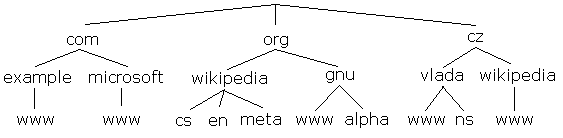
\includegraphics[width=0.85\textwidth]{domeny}
        \caption{Doménový strom.}
    \end{figure}
\end{frame}
\begin{frame}{DNS}
    \vspace{-0.5cm}
    \textbf{\Large \href{https://www.jakfungujedns.cz/}{Jak funguje hledání domény? (link)}}
    \begin{figure}
        \centering
        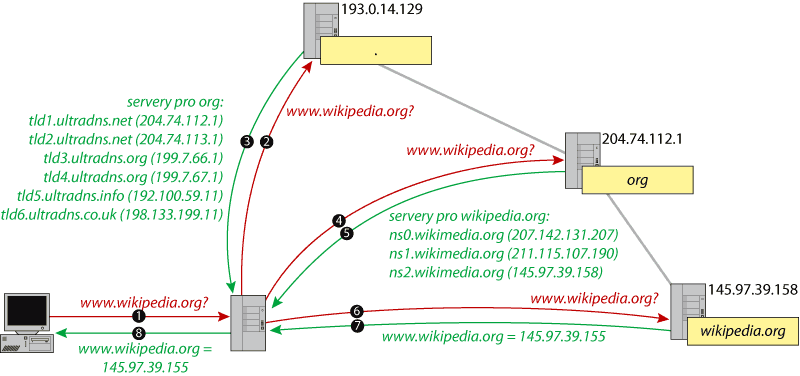
\includegraphics[width=0.85\textwidth]{dns}
    \end{figure}
\end{frame}

\subsection{Sdílení souborů v síti}
\begin{frame}{Sdílení souborů v síti}
    \begin{itemize}
        \item SMB
        \item NFS
        \item GFS
        \item AFS
    \end{itemize}
\end{frame}

\subsection{Vzdálené připojení k počítači}
\begin{frame}{Vzdálené připojení k počítači}
    \begin{itemize}
        \item Telnet
        \item SSH
        \item VNC
        \item RDP
    \end{itemize}
\end{frame}

\finalpagetext{Děkuji za pozornost}
%----------------------------------------------------------------------------------------
\makefinalpage
%----------------------------------------------------------------------------------------
\end{document}
